\documentclass[../main.tex]{subfiles}

\begin{document}
\espacio

  En este capítulo se muestra en detalle la problemática de la investigación.

  \section{Determinación del problema}

  En el contexto de la computación, los procesos a ejecutarse ingresan a una cola de espera que dependiendo del trabajo del procesador, estos procesos pueden tardar un tiempo considerable en ser atendidos, e inclusive desecharse por la excesiva carga de trabajo de la CPU. En las comunicaciones encriptadas, dada la lógica inherente de los procesos de encriptación, los tiempos de ejecución pueden llegar a incrementarse hasta un punto insostenible para un solo procesador. Por lo cual los fabricantes vieron necesario el incremento del número de procesadores a fin de atender los procesos en la cola y evitar desechar tareas por los tiempos de ejecución.

  Desde otro punto de vista, se cuenta con otra alternativa de procesamiento descentralizado mediante la delegación de trabajos a la GPU. Por tanto se verificará la reducción del tiempo de ejecución del algoritmo de encriptación AES mediante la delegación de procesos a la GPU haciendo uso del entorno de programación Python, que cuenta con compatibilidad nativa para la ejecución de tareas en matrices de procesadores CUDA mediante la librería Numba\footnote{http://numba.pydata.org/}.

  \section{Límites y alcances}

  El algoritmo implementado y modificado para la obtención de resultados en CPU y GPU, cumple con la definición de la Publicación de Estándares de Procesamiento de Información Federal 197\footnote{Federal Information Processing Standards Publications - FIPS 197 \cite{report:FIPS_197}}. \cite{report:FIPS_197}. Dicha publicación fué aprobada por el Instituto Nacional de Estándares y Tecnología\footnote{National Institute of Standards and Technology - NIST} después de la verificación en la Reforma de Administración de Tecnologías de la Información\footnote{Information Technology Management Reform} de 1996.

  El relleno de datos de 128 bits cumple con el Estándar de Criptografía de Llave Pública PKCS \#7 plasmado en el reporte RFC 2315 \cite{report:RFC_2315}.

  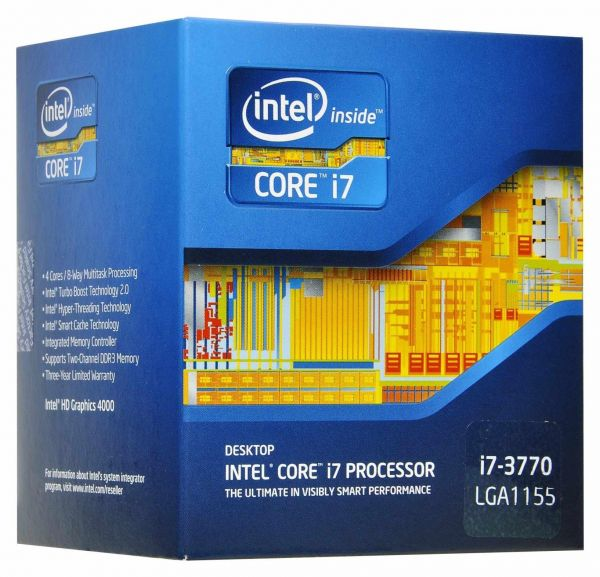
\includegraphics[width=7cm, keepaspectratio]{problema/intel_i7.jpg}
  %------------ TODO cite --------------%
  TODO cite imagen

  En cuanto al hardware, se realiza la comparación de tiempo de ejecución en el microprocesador Intel i7-3770\footnote{https://tinyurl.com/yb3tqpvu} con respecto a la tarjeta gráfica NVidia GTX 650 Ti\footnote{https://tinyurl.com/ycr3kouv}. Lo que representa una comparativa de trabajo simultáneo de 8 núcleos trabajando a 3.4GHz versus 768 núcleos trabajando a 928MHz para las operaciones pasibles a paralelismo.

  
\includegraphics[width=12cm, keepaspectratio]{problema/gtx_650ti.png}
  %------------ TODO cite --------------%
  TODO cite imagen

  El algoritmo utilizado modificado para esta investigación fué escrito por Pablo Caro y es de código abierto, se puede encontrar en la plataforma Github\footnote{https://github.com/pcaro90/Python-AES}.

  Se realizaron modificaciones a este algoritmo mediante la librería Numba\footnote{http://numba.pydata.org/numba-doc/latest/cuda/index.html} que cuenta con decoradores predefinidos que compilan el código a ser paralelizado previa ejecución del programa. Esta librería genera kernels compatibles con plataformas CUDA de distintas arquitecturas.

  El sistema operativo TODO..............

  \bibliografia
\end{document}